%!TEX root = ../main.tex
\subsubsection{The almost everywhere concept}
By construction, Lebesgue integral is not conditioned by single points. In particular a countable set of points does not affect the result. At this point we have to ask ourself if this concept holds also for other properties. Suppose for example that a function satisfy a property except for a countable set of points, can we still apply the theorems that requires such property? The goal of this section is to extend all the previous results of abstract integration to functions defined up to a zero-measure set.

\begin{defn}
	A certain property $P(t)$, with $t\in \Omega$ holds \emph{almost everywhere (a.e.)} in $\Omega$ if:
	$$
		\mu(\{ \ 
			t\in \Omega: \neg P(t)
		\ \})
		=
		0
	.
	$$
\end{defn}

\begin{exam}
	The properties $P(t) = \{\sin(t) \neq 0\}$ and $Q(t) = \{\Ind_\QQ=0\}$\footnote{The function $\Ind_\QQ$, which is the indicator function on the rational number set, is called Dirichlet function.} hold a.e.\ in $\RR$.
	
\end{exam}


\paragraph{Extension of the measurability} The first property that we extend to this context from the general one is measurability:
\begin{defn}
	Let $(\Omega, \mm, \mu)$ be a complete measure space and $(X,\tau)$ a topological space.\\
	A function $f:(\Omega, \mm, \mu) \to (X,\tau)$ is \emph{measurable almost everywhere} in $\Omega$ if both
	$$\text{there exists } \Omega_0 \subset \Omega 
	\text{ such that } \mu(\Omega_0\comp)=0$$
	and
	$$f^{-1}(A) \cap \Omega_0 \in \mm 
	\text{ for all open set } A \subset X.$$
\end{defn}

This say that we require that the preimage of the function, intersected with a set $\Omega_0$ whose complement has zero measure, is still measurable: in this case the function is said to be measurable almost everywhere. In this way the function can be defined (or not) in $\Omega_0\comp$ in any manner without affecting its measurability.

It is easy to see that all the results proved so far, in particular Beppo Levi's, Fatou's and Lebesgue's, can be reformulated for functions defined almost everywhere and they still holds.

\paragraph{Essentially boundedness} In this context it is useful to give another definition of boundedness.
\begin{defn}
	A function $f:(\Omega, \mm, \mu) \to \RR$ is \emph{essentially bounded} if exists $M \geq 0$ such that:
	$$\mu (\{t \in \Omega: |f(t)|>M\})=0.$$
\end{defn}

The concept of almost everywhere allow us to redefine the supremum and the infimum of functions as well.
\begin{defn}
	Let $f:\Omega \to \RR$ be a measurable function.\\
	Then we define its \emph{essential supremum} in $\Omega$ as follows:
	$$\underset{t \in \Omega}{\esssup} f\coloneqq \inf \{M \geq 0 : \, \mu (\{t \in \Omega : |f(t)| > M\}) = 0\},$$
	and the \emph{essential infimum} in $\Omega$ as follows:
	$$\underset{t \in \Omega}{\essinf} f\coloneqq \sup \{M \geq 0 : \, \mu (\{t \in \Omega : |f(t)| < M\}) = 0\}.$$
\end{defn}

\begin{exam}
	Consider for example the Dirichlet function $f(t)=\Ind_\QQ(t)$ with $t \in \RR$. It is bounded and 
	$$
		\sup_\RR f 
		= \max_\RR f 
		= 1
	;
	$$ 
	it is essentially bounded as well, however: 
	$$
		\min \{M\geq 0; \, \lambda( t \in \RR : \Ind_\QQ (t) > 1 )\}
		= 0
	,
	$$
	which means 
	$$
		\esssup_\RR f 
		= \essinf_\RR f 
		= 0 
		\neq \sup_\RR f 
		= 1
	.
	$$ 
\end{exam}

\begin{exam}
	Consider now the following function:
	$$ 
		f(t) = \begin{cases}
			t e^{t^2} \quad & t \in \QQ \\
			\sin(t) \quad & t \in \QQ\comp
		;
		\end{cases}
	$$
	we have: 
	$$
		\esssup_\RR f = 1, 
		\quad \essinf_\RR f = -1, 
		\quad \sup_\RR f = + \infty, 
		\quad \inf_\RR f = - \infty
	.
	$$
\end{exam}


\paragraph{Extension of the continuity} Now we can discuss how also continuity can be defined almost everywhere:
\begin{defn}\label{def:continuity-almost-everywhere}
	Let $(\Omega, \Lc(\Omega),\lambda)$ be a complete measure space where $\Omega \subset \RR^N$ is an open set, and $(X,\tau)$ be a topological space.\\
	A function $f:(\Omega, \mm, \mu) \to (X,\tau)$ is \emph{continuous almost everywhere} in $\Omega$ if both
	$$
		\text{there exists } \Omega_0 
		\subset \Omega 
		\text{ such that } \mu(\Omega_0\comp)
		= 0
	$$
	and
	$$
		f^{-1}(A) \cap \Omega_0 
		\text{  is open for all open set } A 
		\subset X
	.
	$$
\end{defn}
Equivalently a function is continuous a.e.\ if the measure of its discontinuity points is zero.

Observe that if a function is continuous a.e.\ then it's Lebesgue measurable a.e..

\begin{prop}
	Consider two continuous functions $f,g: \RR \to \RR$.\\
	If they coincide a.e.\,
	namely
	$$
		f
		=g 
		\ a.e.
		\text{ with respect to } \lambda
	,
	$$
	then they coincide at any point,
	namely:
	$$
		f(t)
		= g(t) 
		\text{ for any } 
		t \in \RR
	.
	$$
\end{prop}
\begin{proof}
	By contradiction, if there exists $x_0 \in \RR$ such that $f(x_0)\neq g(x_0)$
	then by continuity there exists also a $\delta$ such that
	$f(x) \neq g(x)$
	for all $x \in (x_0 - \delta, x_0 + \delta)$.\\
	But then $\lambda((x_0-\delta,x_0+\delta))=2\delta>0$:
	so there exists an interval of positive measure where the two functions are different, so we have a contradiction.
\end{proof}

\begin{exam}
	Consider again the Dirichlet function $f(t)=\Ind_\QQ(t)$; it is nowhere continuous (it is not continuous a.e. in $\RR$).\\
	However $f = 0 \ a.e.$, so $f$ is equal a.e. to a continuous function. This while the Heaviside function $H = \Ind_{[0,+\infty)}$ is continuous a.e. but it is not equal a.e. to any continuous function. You can prove this. The same consideration can be done for the following: 
	$$
		f(x) 
		\coloneqq \begin{cases}
			\frac x{|x|} & x \neq 0 \\ 0 & x=0
			\end{cases}
	.
	$$
\end{exam}

\begin{exam}
	Consider also the function we seen right before: 
	$$ 
		f(t) = \begin{cases}
		t e^{t^2} 
		\quad & t \in \QQ \\
		\sin(t) \quad & t \in \QQ\comp
		;
		\end{cases}
	$$
	we see that it is not bounded but it is essentially bounded. It is continuous in $t=0$; think whether it is continuous elsewhere!
\end{exam}

\begin{exam}
	At last consider the function $f: \RR \to \RR^\star$ defined in this way:
	$$
		f(t) 
		\coloneqq \begin{cases}
			\arctan(t) & t \in \QQ\comp\\
			+\infty & t \in \QQ \cup [0,+\infty)\\
			-\infty & t \in \QQ \cup (-\infty,0]
			;
		\end{cases}
	$$
	this function is equal a.e. to a continuous function but it's nowhere continuous, it isn't bounded while is essentially bounded.\\
	Same result with 
	$$
		f(t) 
		\coloneqq \begin{cases} 
			\sin(t) & f \in \RR \setminus \QQ \\
			-\infty & t \in \QQ_- \\ 
			+\infty & t \in \QQ_+
			.
		\end{cases}
	$$
\end{exam}

\begin{prop}
	Consider a function $f: (\Omega, \Lc(\Omega),\lambda) \to \RR$, with $\Omega \subset \RR^N$.\\
	As $f$ is Lebesgue measurable, there exists a function $g:\Omega\to \RR$ which is Borel measurable and such that $f = g$ a.e.\ in $\Omega$.
\end{prop}

\paragraph{Extension of convergence theorems} The three convergence theorems, which are the Beppo Levi's or monotone convergence theorem (see theorem \vref{monotone-convergence}), the Fatou's lemma (\vref{fatou-lemma}) and the dominated convergence theorem (\vref{dominated-convergence}), can be trivially reformulated for measurable a.e.\ functions.

In addiction we can prove another theorem for convergence of series of function:

\begin{theo}
	Consider a sequence of functions $\{f_n\}_{n \in \NN} \subset \Lc^1(\Omega, \mm, \mu) \ \forall n \in N$ such that the series $\sum_{n \in \NN} f_n(t)$ converges point-wise $\forall t \in \Omega$, namely:
	$$\sum_{n\in \NN} \int_\Omega|f_n| \,\de\mu < +\infty.$$
	Then $\sum_{n\in\NN} f_n$ converges a.e in $\Omega$ to a function $f\in \Lc^1(\Omega, \mm, \mu)$ and we have:
	$$\int_\Omega f \,\de\mu 
	= \int_\Omega \sum_{n \in \NN} f_n \, \de \mu 
	= \sum_{n\in \NN} \int_\Omega f_n \,\de\mu.$$
\end{theo}
\begin{proof}
	The series $\sum_{n\in \NN}|f_n|$ converges to a non-negative function $g$ and, by Beppo Levi's theorem:
	$$ \int_\Omega \left(\sum_{n\in \NN} |f_n|\right) \,\de\mu = \sum_{n\in \NN} \int_\Omega |f_n| \,\de\mu < +\infty.$$
	Then we say that $\sum_{n\in \NN} |f_n|$ converges a.e. in $\Omega$ to $g \in \Lc^1(\Omega, \mm, \mu)$;	we have that $\sum_{n\in \NN} f_n$ absolutely converges to some $f$ a.e. in $\Omega$, and moreover:
	$$
		\left| \sum_{n=0}^N f_n (t) \right|
		\leq \sum_{n=0}^N |f_n (t)|
		\leq \sum_{n=0}^{+\infty} |f_n (t)|
		= g(t)
	$$
	for almost any $t \in \Omega$ and for all $N$.
	
	Thus we can apply dominated convergence to $\sum_{n=0}^N f_n(t) \to f(t)$. \\
	We have that $f\in \Lc^1(\Omega, \mm, \mu)$, and:
	$$
		\int_\Omega f \,\de\mu
		= \lim\limits_{N \to \infty} \int_\Omega \sum_{n=0}^N f_n(t) \,\de\mu
		= \lim\limits_{N \to \infty} \sum_{n=0}^N \int_\Omega f_n \,\de\mu
		= \sum_{n\in\NN} \int_\Omega f_n \,\de\mu
	.
	$$
\end{proof}
Notice that if $\int_\Omega \sum_{n \in \NN} |f_n| \,\de\mu < +\infty$ then $\sum_{n \in \NN} |f_n|$ is finite a.e. in $\Omega$ and $\sum f_n$ converges a.e. in $\Omega$.

\paragraph{Further results} Here we introduce some other results that can be proven at this state of the theory. First we talk about a useful inequality widely used in probability.
\begin{prop}[Chebyshev's inequality]
	Let $f \in \Lc^1(\Omega, \mm, \mu)$ such that $f \geq 0$ a.e. in $\Omega$, $c>0$.\\
	Then the following inequality holds: 
	$$
		\mu(\{t \in \Omega : f(t) \geq c\})
		\leq \frac 1 c \int_\Omega f \,\de\mu
	.
	$$
\end{prop}
This inequality is trivial if we think to its geometrical meaning.
\begin{figure}[htpb]
	\centering
	\tikzset{every picture/.style={line width=0.75pt}} %set default line width to 0.75pt        

	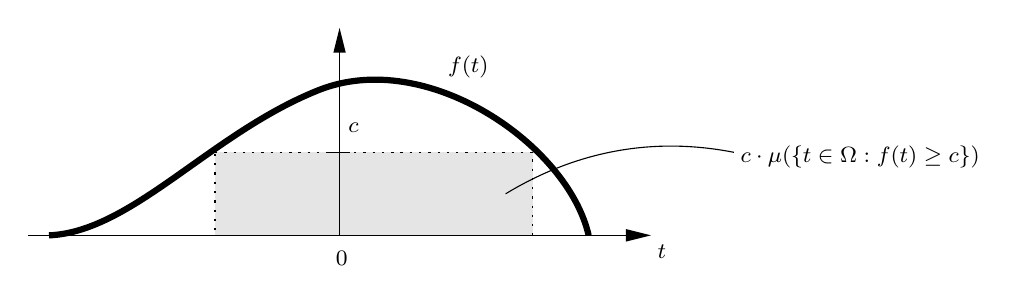
\begin{tikzpicture}[x=0.75pt,y=0.75pt,yscale=-1,xscale=1]
	%uncomment if require: \path (0,257); %set diagram left start at 0, and has height of 257

	\draw (70,170) -- (368,170);
	\draw [shift={(370,170)}, rotate = 180] [fill={rgb, 255:red, 0; green, 0; blue, 0 }  ][line width=0.08]  [draw opacity=0] (12,-3) -- (0,0) -- (12,3) -- cycle;
	\draw (220,170) -- (220,72);
	\draw [shift={(220,70)}, rotate = 90] [fill={rgb, 255:red, 0; green, 0; blue, 0 }  ][line width=0.08]  [draw opacity=0] (12,-3) -- (0,0) -- (12,3) -- cycle;
	\draw [line width=2.25] (80,170) .. controls (120,168.36) and (158,120.64) .. (210,100) .. controls (262,79.36) and (330,126.36) .. (340,170);
	\draw  [fill={rgb, 255:red, 0; green, 0; blue, 0 }  ,fill opacity=0.1 ][dash pattern={on 0.84pt off 2.51pt}] (160,130) -- (313,130) -- (313,170) -- (160,170) -- cycle;
	\draw (300,150) .. controls (334,129.36) and (371,122.36) .. (410,130);
	\draw (225,130) -- (215,130);

	\draw (217,176.4) node [anchor=north west][inner sep=0.75pt]  [font=\footnotesize]  {$0$};
	\draw (271,82.4) node [anchor=north west][inner sep=0.75pt]  [font=\footnotesize]  {$f(t)$};
	\draw (223,114.4) node [anchor=north west][inner sep=0.75pt]  [font=\footnotesize]  {$c$};
	\draw (412,125.4) node [anchor=north west][inner sep=0.75pt]  [font=\footnotesize]  {$c\cdot \mu ( \{t\in \Omega:f( t) \geq c\})$};
	\draw (372,173.4) node [anchor=north west][inner sep=0.75pt]  [font=\footnotesize]  {$t$};
	\end{tikzpicture}
\end{figure}
\FloatBarrier
\begin{proof}
	Consider the following chain of inequalities:
	$$
		\int_\Omega f \, \dmu 
		\geq \int_{\{t \in \Omega : \, f(t) \geq c\}} f \, \dmu
		\geq c \cdot \mu(\{t \in \Omega: \, f(t) \geq c\})
	.
	$$
\end{proof}

Here another useful tool:
\begin{prop} \label{integral-inequality-sigma-finite}
	Let $(\Omega, \mm, \mu)$ be a $\sigma$-finite measure space.\\
	Consider two measurable functions $f,g: \Omega \to [0, +\infty]$ such that:
	$$
		\int_E f \, \de \mu \leq
		\int_E g \, \de \mu
		\quad \text{for all } E \in \mm
	,
	$$
	then $f\leq g$ almost everywhere in $\Omega$.
\end{prop}

Lastly we present a simple yet useful result:
\begin{theo}[Vanishing lemma]\label{vanishing-lemma}
	Let $f\in \Lc^1(\Omega, \mm, \mu)$ such that $f\geq 0$ a.e. in $\Omega$.
	$$
		\text{If }\int_\Omega f \,\de\mu = 0\text{ then }f = 0 \text{ a.e. in } \Omega.$$
\end{theo}
\begin{proof}
	Take the following set for each $n \in\NN_0$:
	$$
		E_n 
		= \{t \in \Omega : f(t) \geq \frac 1 n \} \in \mm
	.
	$$
	Then:
	$$ 
		0 
		= \int_\Omega f \,\de\mu 
		\geq \int_{E_n} f \,\de\mu 
		\geq \frac 1 n \mu (E_n)
		\quad \forall n \in \NN_0
	.
	$$
	Thus $\mu(E_n) = 0$ for all $n \in \NN_0$.
	
	Now suppose there exists $t \in \Omega$  such that $f(t) > 0$.\\
	Then it exists $n_0 \in \NN$ such that $f(t) \geq \frac 1 {n_0}$, and so
	$$t \in E_{n_0}\subset E \text{ where } E = \bigcup_{n\in \NN_0} E_n.$$\\
	Thus $\{t\in \Omega : f(t) > 0\} \subseteq E$, so: 
	$$\mu (E) \le \sum_{n \in \NN} \mu(E_n) = 0.$$
\end{proof}


A brief final remark: consider $\Lc^1(\Omega, \mm, \mu)$ and define $d(f,g) \coloneqq \int_\Omega |f,g| \,\de\mu$. Notice that such function is not a metric: indeed, by the vanishing lemma, $d(f,g)=0 \implies f=g$ not everywhere, but \textit{almost} everywhere $\in \Omega$.\\
To solve the problem, we consider the following equivalence relation: $$f \sim g \iff f=g \text{ a.e. in } \Omega$$
Take the quotient set $X_1 \coloneqq \frac{\Lc^1(\Omega, \mm, \mu)}{\sim}$. Then $d$ is a metric in $X_1$.

%
%
%
%
%\subsection{Comparison between Lebesgue and Riemann integral}
%
%In this section we will consider the space $(\RR, \Lc(\RR), \lambda)$, and we will focus on intervals.
%
%\begin{theo}
%	Let $a,b \in \RR: a<b$, $f:(a,b) \to \RR$ bounded. \\
%	Then $f$ is \emph{Riemann-integrable} in $(a,b)$ if and only if $f$ is continuous a.e. in $(a,b)$.
%\end{theo}
%
%Notice that $\Ind_{\QQ \cap (a,b)}$ is not Riemann integrable, because it is nowhere continuous. But $\Ind_{\QQ \cap (a,b)}=0$ a.e. in $(a,b)$, it is Lebesgue-integrable, and $\int_a^b \Ind_{\QQ \cap (a,b)} \dlam =0$.
%
%More in general, if $f: (a,b) \to \RR$ is Lebesgue-measurable and bounded, then $f$ is Lebesgue integrable.
%
%\begin{theo}
%	Let $f:(a,b)\subset \RR \to \RR$ be bounded and continuous a.e. in $(a,b)$. Then:$$ \underbrace{\int_a^b f(t) \,\dt}_{Riemann}
%	= \underbrace{\int_a^b f(t) \,\dlam}_{Lebesgue}$$
%\end{theo}
%
%For the proof see k-f pp 309-310.
%
%Let us now focus on improper Riemann integrals, where $f$ and/or the integration domain is unbounded. We have: %rewrite
%\begin{theo}
%	Let $f: (a,b) \subseteq \RR \to \RR$, with $a,b\in \RR^\star : a< b$.
%	
%	If $f$ is Riemann integrable in $(a,b)$ in the improper sense and it changes its sign at most a finite number of times, then	$f$ is Lebesgue integrable in $(a,b)$ and the two integrals coincide.
%\end{theo}
%
%\begin{proof}
%	Suppose $f>0$. We can find two sequences, $\{a_n\}_{n\in \NN}$ and $\{b_n\}_{n\in \NN}$, such that $a_n < b_n$, $a_n \downarrow a$, $b_n \uparrow b$, and $(a,b)=\bigcup_{n\in \NN} (a_n,b_n)$.
%	
%	Suppose $f$ is bounded on $(a_n,b_n) \ \forall n \in \NN$.\\
%	Therefore $f$ is Riemann integrable on each $(a_n,b_n)$ and we have:
%	\begin{align*}
%	\underbrace{\int_{a_n}^{b_n} f(t) \,\dt}_{Riemann}
%	&= \underbrace{\int_{a_n}^{b_n} f(t) \,\dlam}_{Lebesgue}
%	\quad \forall n \in \NN
%	\intertext{Set $F_n \coloneqq \bigcup_{j=0}^n (a_j,b_j)$ and $f_n \coloneqq f \Ind_{F_n}$. $f_n \uparrow f$ and, using Beppo Levi's theorem, we have:}
%	\int_a^b f(t) \,\dlam
%	&= \lim_{n \to \infty} \int_a^b f_n(t) \,\dlam
%	= \lim_{n \to \infty} \int_{a_n}^{b_n} f(t) \,\dlam
%	\intertext{By definition of Riemann improper integral, we have:}
%	\int_a^b f(t) \,\dt
%	&= \lim_{n \to \infty} \int_{a_n}^{b_n} f(t) \,\dt
%	\end{align*}
%	Putting all together, we get the thesis.
%\end{proof}
%
%Notice that there functions which are Riemann- but not Lebesgue-integrable.
%\begin{exam}
%	$$f(t)=\frac {\sin t}{t} \quad t \in (0,+\infty)$$
%	$f$ is Riemann-integrable: $\lim\limits_{a \to +\infty} \int_0^a f(t) \,\dt$ exists. However:\todo{Explain better?}
%	$$ \int_0^{+\infty} \left| \frac{ \sin t}{t} \right| \dlam
%	= \int_0^{+\infty}\frac 1 t \dlam = +\infty $$
%	Thus $f$ is not Lebesgue-integrable.
%\end{exam}
%
%%reload
%\medskip
%\begin{exam}
%	Consider the following function:
%	$$f(t)\coloneqq\begin{cases}
%	\sin(t) & \text{if } t \in \RR \setminus \ZZ \\ 
%	+ \infty & \text{if } t \in \ZZ^+ \\ 
%	- \infty & \text{if } t \in \ZZ_-	
%	\end{cases} $$
%	
%	$f$ is essentially bounded and continuous a.e. in $\RR$, and $f(t) = \sin(t)$ a.e. in $\RR$.
%\end{exam}
%
%\medskip
%\begin{exam}
%	Consider the following function:
%	$$f(t)\coloneqq\begin{cases} 
%	\sin(t) 		& \text{if } t \in \left[0,1\right]\cap \left(\RR \setminus \QQ \right) \\
%	+ \infty 	   &  \text{if } t \in \left[0,1\right]\cap \QQ
%	\end{cases}$$
%	
%	$f$ is nowhere continuous, bounded, and measurable. Then that $f$ is Lebesgue integrable, hence $\int_0^1 f(t) \,\dlam$ exists finite.
%	
%	Indeed, $f(t) = \sin (t)$ $a.e.$ in $\left[0,1\right]$, thus:
%	$$\int_0^1 f(t) d \lambda =\underbrace{\int_0^1 \sin t \,\dlam}_{Lebesgue}
%	=\underbrace{\int_0^1 \sin t \,\dt}_{Riemann}$$
%\end{exam}
%
%Notice that there are some functions which are $\Lc$-integrable but they are not even equal a.e. to a R-integrable function. For instance, consider the characteristic function of a generalized Cantor set.
